\documentclass[sigconf]{acmart}

\usepackage{hyperref}

\usepackage{endfloat}
\renewcommand{\efloatseparator}{\mbox{}} % no new page between figures

\usepackage{booktabs} % For formal tables

\settopmatter{printacmref=false} % Removes citation information below abstract
\renewcommand\footnotetextcopyrightpermission[1]{} % removes footnote with conference information in first column
\pagestyle{plain} % removes running headers

\begin{document}
\title{Big Data Mental Health Monitoring: A Private and Independent Approach}


\author{Neil Eliason}
\affiliation{%
  \institution{Indiana University}
  \city{Anderson} 
  \state{Indiana} 
  \postcode{46017}
}
\email{nreliaso@iu.edu}

% The default list of authors is too long for headers}
\renewcommand{\shortauthors}{N. Eliason}


\begin{abstract}

Big data holds great promise in a number of fields, and mental health treatment is no exception. Effective big data applications have been developed for every stage of treatment, but not without difficulties. This is particularly true for passive monitoring using smartphones. While it provides improved resolution of consumer behavior, it has complications with privacy and implementation connected with use of commercial software and streaming data. This project created an open source program which uses discrete exported data from smartphones to implement passive monitoring in a way that promotes consumer control of their data and independence from commercial interests. A working program which parses and analyzes smartphone data was created to demonstrate concepts, but would benefit from further development of parser options, analyses, and input/output file management in the future.

\end{abstract}

\keywords{i523, passive monitoring, open source, mental health treatment, big data}


\maketitle

\section{Introduction}

Can big data contribute to the treatment of mental illness? Are there any unique issues that hinder big data being used for mental health treatment? Big data has certainly gained the reputation of being a formidable remedy for analytical problems. Corporate empires such as Google, Facebook, and Amazon were built on a foundation of handling and managing big data, and scientists have explored everything from the structure of galaxies to the language of our genes using the power of big data. Perhaps it can work such wonders in the field of mental health as well.

\subsection {What is Big Data?}

First of all, what is big data? This proves to be a difficult question to answer, as definitions vary based upon industry and often shift as technology evolves and adapts. However, there are three generally accepted traits of big data: high volume (amount of data), high velocity (rate of data creation), and/or high variety (number of data sources). It is when these data traits become increasingly extreme, and require non-traditional analytic methods to extract insights, that it becomes big data \cite{bdconcepts}. 

The need for big data analytics has arisen, partly because data storage capabilities have increased at a faster rate than that of data processing. This paired with the proliferation of data collecting devices creates a surplus of stored data that is growing faster than it can be processed traditionally. This drives the demand to develop new ways to extract insights from big data \cite{bdsurvey}. 

Big data approaches can be applied to every stage of the data life cycle. Unworked data can be extracted from varied and possibly streaming sources and cleaned and organized automatically. Then predictive analytics can be applied to identify patterns in the data, relying on either regression techniques or machine learning. These approaches attempt to scale these extreme data sets to the level of human insight by reducing noise and identifying patterns via automation and intelligent algorithms \cite{bdconcepts}.

\subsection{Mental Health Treatment}

Mental illness has been a prevalent issues for all societies worldwide. It has been estimated that 29.2 \% of the world population will personally struggle with mental illness, and that 17.6 \%  had a mental illness in 2014 \cite{worldprev}. In the United States, 17.9 \% of the population was estimated to have mental illness \cite{nihmstats}. The negative impact of these disorders is high. It is estimated by the Center for Disease Control and Prevention that 36,035 Americans died by suicide and 666,000 visited acute care for harm to self in 2008 \cite{cdcsuicide}. 1,947,775 Americans drew social security/disability due to a psychotic or mood disorder according to the Social Security Administration in 2013, making up around 19 \% of recipients \cite{ssarecipients}. In 2002, mental health issues are estimated to have had \$ 100 billion negative effect on the US economy \cite{nihmstats}, and over 12,000 facilities were providing mental health services in 2015 in the United States \cite{n-mhss2015}. It is evident given the scale of the negative impact mental illness has on individuals and societies, that effective solutions are needed.

Services provided to meet this need vary depending on a variety of factors, but typically involve a screening and assessment process \cite{apapractscreeassess}, assignment of interventions \cite{samhsatx}, and monitoring of treatment progress \cite{progressmonitoring}. Mental health screening is an initial contact that takes a relatively succinct amount of information and seeks to guide the person towards the right services. They are designed to not be time consuming or overly invasive to distribute them to a wide group of people. Assessment is more comprehensive, with the goal of identifying primary mental health needs and clinical diagnoses for the purpose of informing treatment decisions \cite{apapractscreeassess}.

After the treatment team has determined a person's needs and diagnosed clinical disorders, appropriate interventions are chosen, and added to the person's treatment plan. Typical services are talk therapy which targets developing positive change strategies, medication management which seek to manage symptoms through psychiatric drugs, and case management and related support services which assist in coordinating details of their care and applying skills learned in treatment \cite{samhsatx}. 

Treatment monitoring is where clinicians assess if treatment is resulting in positive change for the person receiving treatment. Without this feedback, it is easy for clinicians to lose sight of how the person is doing. Though most clinicians have methods of assessing progress, it can be difficult to do so objectively \cite{progressmonitoring}.

The majority of the activities of mental health treatment involve gathering data about the treatment consumer and extracting clinically meaningful insights. This frequently generates considerable amounts of data, which is often from a variety of sources, thus making big data approaches appropriate for consideration.

\subsection{Big Data Mental Health Applications}

Given the problem-solving potential of big data analytics, many researchers have explored ways to apply these techniques to the problem of treating mental health difficulties. Providing quality mental health treatment involves considerable information gathering and insight extracting work, thus making big data techniques relevant for every stage of the treatment process. 

\subsubsection{Screening and Assessment}

Mental health screening typically is the first contact people have with mental health  services, and serve the important role of identifying mental health needs at a larger scale. Thus screening methods that are easy to implement and capture information from a large group are ideal. Many big data approaches to this problem have been attempted, often using data found on social media. This provides a large, if not messy dataset, but the accuracy of these methods was found to be better than that typical of primary care providers, but worse than self-reporting tools \cite{detectdepressionsocialmedia}.

Assessment and diagnosis is more information intensive and traditionally requires the skills of a highly trained clinician. Many studies have looked at how to streamline that task by using data gathered through data mining and natural language processing to group people into diagnostic categories using machine learning techniques. While this approach has some success, it has not demonstrated more accuracy than traditional assessment methods, thus suggesting that it may primarily serve an assisting role for the time being. Related to big data assessment techniques, outcome prediction using machine learning has been used to attempt to identify a person's likely treatment trajectory, given certain factors. These predictive models sought to connect risk factors with negative outcomes, and was able to do so with a fair degree of accuracy (69\% to 99\%). However, sample sizes were small, so further research is needed to fully assess their efficacy \cite{machinelearnbipolar,bigdatabipolar}.

\subsubsection{Interventions}

Treatment interventions are the actual delivery of services, such as therapy or medication management. They are very personalized and focus on facilitating positive change in the treatment consumer. Thus there are not as many Big Data opportunities, as intervention itself does not generate massive amounts of data. However, certain web-based interventions could use big data techniques by delivering interactive services to a large number of consumers at one time, thus requiring specialized analytic techniques to respond to user input \cite{bitreview,webtx}. 

\subsubsection{Treatment Monitoring}

Just as screening and assessment provide the clinician with information to guide what treatment they are to receive, treatment monitoring aims to inform the clinician on the efficacy of treatment. Though this is just as important, it is often difficult to be objective and to engage the consumer in providing needed information. Active monitoring via smartphones has been explored as a possible solution. Through apps or text messages, a consumer is reminded of treatment goals and symptoms are assessed in real time. This data can be generated multiple times a day, and takes a variety of forms, which indicates a possible big data opportunity \cite{bitreview}.

Passive monitoring is a similar approach, but instead of relying on consumers to actively respond, it gathers data from them throughout the day. This data can be collected in a number of ways, including smartphones and wearable devices. Many studies have paired this active monitoring data with machine learning techniques to create predictive models \cite{bitreview}. One example of this is an initiative to develop a program which can identify whether someone is experiencing symptoms of bipolar disorder from input on their smartphone such as data from the devices sensors or from keyboard input \cite{forbesresearchkit}. The app is being developed in Apple's ResearchKit, which is an open source medical research application development tool \cite{researchkit}.

While these techniques are promising, implementing them can be challenging, given the variety of data sources involved from different devices. It is also difficult to test the approaches with consumers, due to lack of engagement \cite{bigdatabipolar}. Provision of technical support and clinical engagement concerning passive monitoring techniques has shown to help improve consumers' level of engagment \cite{bithuman}.

\subsection{Barriers to Big Data for Mental Health Treatment}

Every stage of treatment can benefit from big data applications to differing degrees. The screening and assessment process is the most information intensive stage, and thus has received considerable attention from Big Data application research. These efforts have had some success, though they have not surpassed traditional methods, and have not been validated on larger samples sizes \cite{bigdatabipolar}.

However, treatment monitoring, particularly passive monitoring is considerably information intensive as well, and can potentially produce datasets with more volume, variety, and velocity than initial assessment services. As seen above, development of these approaches appears to be slower, due to a number of issues inherent in many Big Data applications, which are accentuated in passive monitoring. For this reason development of this approach has been slower, though it has elicited considerable interest and discussion \cite{bitreview}.

A primary concern is that privacy will be compromised for persons who participate in treatment that utilizes big data techniques, particularly passive monitoring. The use of commercial software for data analysis often requires that the analytics company process the data themselves rather than the treatment provider. This is especially true of mobile device apps, which usually take data, and send it back to their own servers to be processed. These applications do not necessarily have the same privacy rules that medical records due concerning protected health information \cite{bigdatabipolar}. A key part of privacy is one's ability to control what information about them goes where, and to prevent unwanted information from being shared \cite{privacy}.With streaming personal data from smartphones, consumers begin lose some of their privacy, because they lose control of their data. As it is constantly being sent to the treatment provider, and requires action on the part of the consumer for it to stop, the person has sacrificed some of their privacy in order to receive this service. Though this is a common trade off in medical and mental health contexts,research indicates that people prefer to have more control of the private data, and that they want to be able to share it in portions, rather than have to share all of it \cite{privacypreference}.

Another issue related to using activity monitoring in mental health treatment is that the variety of competing smartphone and wearable sensor companies creates an environment with plenty of human behavior Big Data, but it is not easy to integrate. This  data is stored on separate private databases and each company has fiscal motivations to resist collaboration. Thus the product which a treatment provider intends for use as a clinical tool, is also being used for a commercial purpose, and to create a comprehensive application which is not encumbered by the independent economic interest of a private business is difficult \cite{openinfrastructure}.

Some companies  attempt to avoid this by providing some open source products. Open source software is freely distributed, can be modified and integrated into other software, the source code is available, and it is not associated with any specific product. Benefits of such code is that they can be improved by a large number of programmers, they can be widely implemented, and it is not tied to any product or corporation \cite{opensourceinit}. An example of such as Apple's ResearchKit \cite{researchkit}.  However, though the product is free, it is still tied to the company's resources, in this case Xcode \cite{setupresearchkit} Though some development can be done freely, Apple controls this, and extensive work cannot be easily distributed without paying for a developer account \cite{appledeveloper}. While there are some truly free open-source software solutions for mental health, they tend to target administrative problems, rather than treatment itself \cite{topopenmental}.

\subsection{Open Source and Discrete Data Transfer}

A true open source big data solution could make passive monitoring an ethical and workable tool for mental health treatment. A program written in the open source programming language Python would be free of corporate entanglements and costs, but would benefit from the massive amount of documentation, packages, and ready-made code produced by the Python community \cite{pythonfoundation}. Run on open source Ubuntu Linux \cite{ubuntu} installed on open source Oracle Virtual Box \cite{virtualbox}, such a program would be independent of commercial interests, completely reproducible, and free of charge. Besides these direct benefits, open source programs often have performance and security advantages of commercially developed products \cite{opensourcereasons}.

The data source for the passive monitoring would still be smartphones, but instead of using commercially provided apps for analysis, the data would be extracted and analyzed using the open source based program. The iPhone step count data collected by the built-in accelerometer, and stored in the Health App can be exported via email as an xml file \cite{howtoexporthealth}. Though this method losses the benefits of streaming data, it increases the consumers' control over their data by making data transfer definite and discrete. Instead of agreeing to install an app on their device which will track their behaviors forever unless they ask for data to stop streaming or the app is uninstalled, the consumer can agreed to provide a defined amount of information now, and may do so again later. As the Health export file stores all detected steps, no data is lost, it is just not seen in real-time. This would still provide useful information for treatment monitoring purposes. 

Using this method also allows for the steps data of numerous people to be parsed and analyzed in an automated fashion, which would be necessary from a mental health treatment perspective, as numerous consumers data would need processed. As datasets increase, some way of address the increasing extremity of the data needs to occur. There are other approaches that would be insightful, but this approach is a good fit when the output is a file for each individual participant, rather than aggregate date about a group.

\subsection{Thesis}

Private and independent passive monitoring can be utilized in mental health treatment by leveraging open source programming tools to analyze aggregate movement data provided from smartphones in discrete amounts. This approach avoids the cost and entanglements of commercial software and wearable technology, as well as increases consumer control over their personal data. 

\subsection{Project Goals} This project attempts to demonstrate this concept by developing a simple open-source program written in Python which can perform full data life cycle analytics on automatically collected iPhone Health App data. The program was designed to accommodate Big Data by automatically iterating over multiple files without user input.

\section{Methods}

\subsection{Design}

This current research utilized the Python programming language to develop a program which could parse, analyze, and report clinically relevant information from a folder of exported individual iPhone 6 Heatlh App data files. This program consisted of four sub-programs: acceleparser.py, Tables.py, Visualizations.py, and makefile.py. Also included with the program code was a folder named iPhoneData which contained the test xml files, and a bash script named make\_install.sh which installed program packages. 

The acceleparser.py program which imports the xml file and parses it using the ElementTree python package. The xml file is imported and parsed into a tree structure. It then iterates through the tree and appends date/time data and steps data to corresponding lists. Those lists are then used to create a dataframe using the pandas python package, which is then returned. 

The Tables.py program takes the dataframe returned from acceleparser.py, and formats it for display and for use by the Visualizations.py program. Tables.py consists of two functions, stepsBYdata and stepsBYweekday. The stepsBYdata function formats the dataframe to show the total steps for each date using the pandas groupby functionality. The stepsBYweekday function formats the dataframe to display the mean steps for each date in columns of weekdays, and rows of weeks labelled by the first Monday's date. This was accomplished using pandas pivot table functionality to aggregate the mean function over the dataframe, and then a new dataframe was made with the weekday columns. Each function returns a dataframe object.

The Visualizations.py program takes input dataframes from either acceleparser.py or Tables.py, and returns graphs. Visualizations.py consists of two functions. The stepsBYdateGraph function takes the dataframe created by the stepsBYdate function of Tables.py and creates a time series line graph using matplotlib.pyplot python package. The stepsBYweekdayGraph function takes the dataframe returned  by acceleparser.py, and creates a list of mean steps for each day of the week and a list of days of the week. From these lists, a bar graph of the mean of steps for each day of the week is generated using matplotlib.pyplot.

The makefile.py program iterates over the xml files stored in the iPhoneData folder, and for each file ran the acceleparser.py program, and directed that dataframe to the Tables.py and Visualizations.py programs to output the table and graphs. The table was then saved as a txt file and the graphs saved as pdf, each named by which iteration the original file was in the for loop.

This program utilized the module design of small sub-programs to provide ease of customization and expansion of program features. Later functions can be added to their appropriate subprograms, and the makefile.py modified to include the new function, and thus generate a new report. Multiple reports could even be added to the makefile.py, and executed when called.

\subsection{Data}

The test data consisted of xml files exported from the Apple Health App on iPhone 6. To export the data, the export health data option was selected in the app, which compiled as export.zip. This file was then emailed to researcher and the file unzipped as folder named apple\_health\_export. This folder contained two files, export.xml and export\_cda.xml. The export.xml file contained the steps data, and was renamed ``Client1'' and placed in the hid312 folder in the i523 class google drive site \cite{testdata}. 

Health data was exported from two devices, which contained a variety of data, but only date/time and step count data were used in this project. The xml files were 5.58 MB and 8.33 MB in size, containing 203 days and 888 days of steps data respectively. Data was also tested from iPhone 8  models, but the program would not parse the files, and thus were excluded from the final test set.

\subsection{Analyses}

Basic descriptive statistics were utilized to explore patterns of step activity over time. Daily step counts were organized in table fashion by day of the week columns and rows of weeks. Visual analyses consisted of a bar graph of the mean steps taken for each day of the week and of a time series line graph of daily steps taken over time. These analyses were chosen to show basic patterns in data in a way which could be quickly assimilated. 

\subsection{Specifications}

Project development and testing was done in Ubuntu Linux operating system version 16.04 (download available at \cite{ubuntu}) installed on an Oracle Virtual Box Graphical User Interface (download available at \cite{virtualbox}). Code was written in Python version 3.5.2 (download available at \cite{python3.5.2}) installed within pyenv Python Version Management System (download available at \cite{pyenv} per installation instructions available here \cite{cloudmeshpyenv}). External Python libraries utilized in project were pandas, matplotlib, and numpy (download available from the Python Package Index \cite{pypi}). With this configuration, it was necessary to install tk-dev system wide prior to creating pyenv virtual python environment (instructions found at \cite{tk-dev}), and to install python3-tk within the virtual python environment in order to utilize matplotlib.pyplot. Completed source code can be found at Neil Eliason's bigdata-i523 github repository \cite{sourcecode}. 

\subsection{Procedure}

Program tests were done per instructions found in the README.md file of the project sourcecode \cite{sourcecode}.

\section{Results}
After executing the program, the output was one txt file and two pdf files for every one input xml file. Thus, for the test data of two xml files, six files were created. All files were generated in the code directory from which makefile.py was ran. 

The txt file contained a table with columns of daily steps for each day of the week and rows labelled as the date of the first day of the week, with each week starting on Monday. The file name was determined by where in the order the original xml data was parsed in the program iteration. For example, the output txt file for the first parsed xml file would be named ``Client1.txt''.

\begin{table*}[htb]
\caption{Output table of daily steps by day of the week}
\includegraphics[width=\textwidth]{images/Client1Report.pdf}
\end{table*}

The pdf files were graphs of certain descriptive analytics based on the parsed data. The first was a time series line graph of daily step information for the whole time period of the xml file. The second was a bar graph of the mean steps for each day of the week of the whole time period of the dataset. These files were named similarly to the above txt file, with each file named according to its order in the iteration. For example, the first xml file parsed would generate ``Client1StepsByDate.pdf'' for the first graph and ``Client1StepsByDayOfWeek.pdf'' for the second.

\begin{figure}[htb]
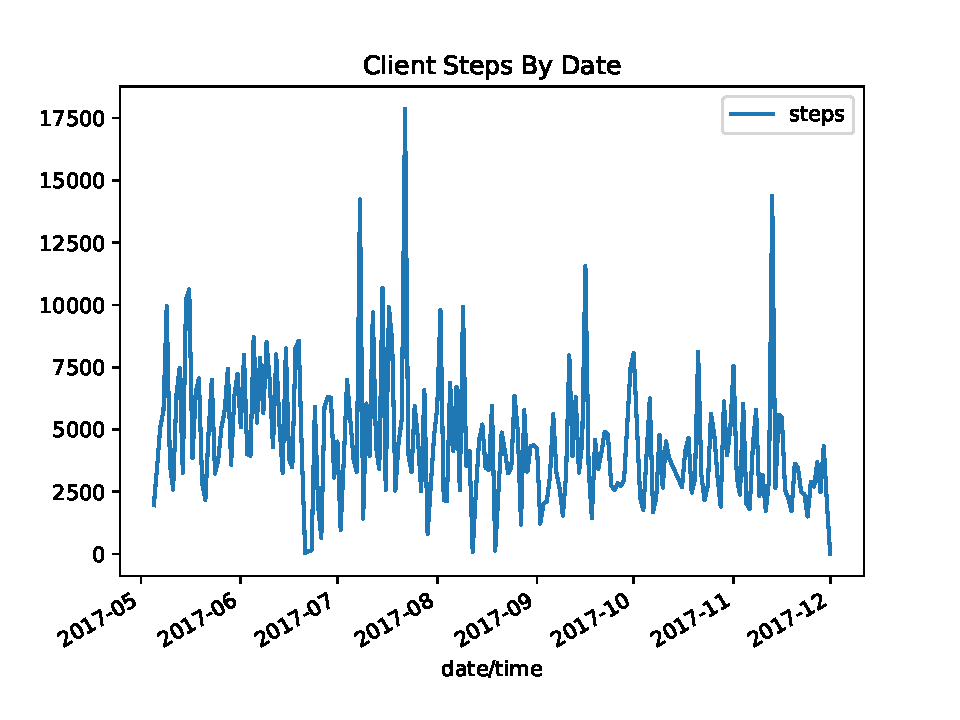
\includegraphics[width=1.0\columnwidth]{images/Client1StepsByDate.pdf}
\caption{Output graph of time series of daily steps}
\end{figure}

\begin{figure}[htb]
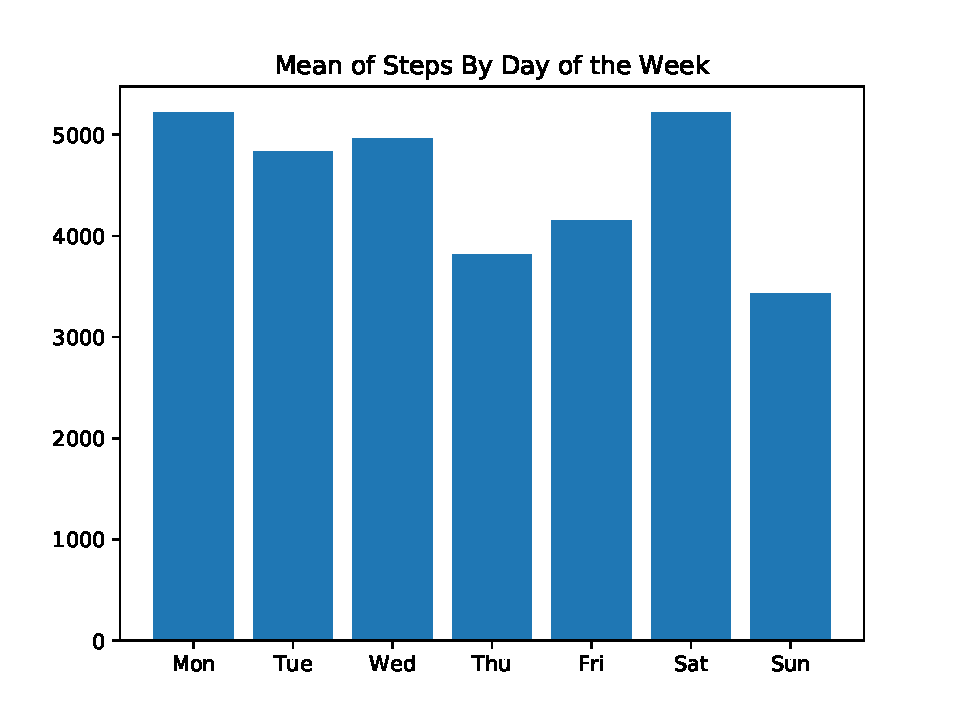
\includegraphics[width=1.0\columnwidth]{images/Client1StepsByDayOfWeek.pdf}
\caption{Output graph of mean steps for each day of the week}
\end{figure}



\section{Discussion}

\subsection{Project Goal Assessment}

The goal of this project was to address the common issues of privacy concerns and ease of implementation that hinder applying Big Data techniques to Mental Health Treatment. The strategy was to write a program that leveraged open source software, used smartphone data provided by the consumer in discrete and definite ways, and allowed for applications in a Big Data setting.  

\subsubsection{Open Source}

The source code for the program was written in Python 3.5.2, and utilized the pandas, matplotlib, and numpy packages to perform data cleaning, organization, and visualiztion. All these resources are available online free of charge, and with substantial technical support and documentation. By following the installation instructions found in the README.md, this program can be installed on the open source Ubuntu operating system on Virtualbox, thus making the program configuration reproducible on any standard operating system with sufficient hardware. This allows for distribution in various settings with no cost or input from outside commercial interests. The project successfully created a working program using open source programs.

\subsubsection{Discrete Data Delivery}

Data was exported from the iPhone Health app, and emailed to the researcher as a single file. By using a discrete dataset, the person providing the data did not have to install invasive apps on their phone or agree to releasing information for an indefinite amount of time. They made the decision to provide a set amount of data, and can make a subsequent decision to do so at a later time, but they do not have to make a decision to stop sharing the data. They must be active to share in the future, rather than needing to be active to stop sharing. The project successfully utilized discrete data as the data source for the program.

\subsubsection{Big Data Informed}

By utilizing a design that iterates the program through a folder of data files, one command from the terminal can theoretically produce the output files for hundreds of consumers. This functionality is necessary when dealing with big data, as it would be incredibly tedious, if not impossible to do such a task through the graphical user interface. While the program was designed to be useable with big data, testing was not done with a dataset which would qualify as big data. Also, no big data analytics, such a machine learning were utilized. The project successfully developed a starting platform for big data analytics, but needs further development.

\subsection{Thesis Assessment}

This project was able to create an open-source program which analyzes readily available behavior data from smartphones provided in discrete samples, rather than streaming. While the project goals were met, how do they relate to the thesis? Do these results support the thesis that open-source programs and discrete data collection address issues of consumer data control and flexible implementation of passive monitoring in mental health?

The diverse selection of technology companies fighting for a larger piece of a lucrative market share certainly creates numerous products which could be used for passive monitoring applications. However, corporate competition hinders collaboration and integration of these tools into a comprehensive mental health Big Data approach \cite{openinfrastructure}. Also, by utilizing commercial software, data is not always guaranteed to be protected, and may be gathered from apps and analyzed by the corporation for business purposes \cite{bigdatabipolar}. By utilizing completely open source products for the project,to analyze multiple persons' accelerometer data from a popular smartphone device, this project demonstrates that a corporate interference free approach to passive monitoring is possible. By avoiding corporate interference, the implementation of this approach is completely flexible and the fate of data is clear and transparent encouraging safety of consumer data.

Much attention has been given to the power of streaming data, which is not unwarranted. In the context of passive monitoring, streaming data can provide an incredible level of information resolution about a consumer's behavior \cite{openinfrastructure}, and safety planning and monitoring could utilize such approaches to identify when someone may be more symptomatic and in danger \cite{bitreview}. However, these approaches to passive monitoring remove control of the data from the consumer, and force them to take action if they want that data sharing to stop. Given that people generally prefer to have greater control over what data is shared and when \cite{privacypreference}, this may contribute to some of the lack of engagement found in some implementations \cite{bitreview}. By using discrete  streaming data, this project allows for consumers to have more control over their personal data, while still benefiting from the clinical insights afforded by passive monitoring. Another ancillary benefit of utilizing discrete data transfer is that it actually facilitates more interaction between the consumer and the service provider about the health data. This can provide opportunities for insight development for the consumer by increasing awareness of their behaviors and activity.

\subsection{Limitations and Future Directions}

This project's aim was to develop a prototype passive monitoring program using open source and discretely provided consumer data that could be utilized with Big Data. While this was accomplished, the actual work the program does is fairly basic. The hope would be for more robust and effective models of passive monitoring to be built expanding on these approaches. As it is, the current project has the following limitations.

\subsubsection {Depth of analysis}

As seen above, a number of powerful analytic techniques are available for use on big data sets. From traditional inferential statistics, to machine learning, to advanced visualizations, more extensive analytics could provide increased insight from this data. By including another variable, such as reported mood, hours of sleep, etc. machine learning techniques could attempt to identify patterns between the variables. This particular data may especially benefit from exploring patterns at different levels of resolution, attempting to identify patterns in activity based on time, day, week, or month, and pair this with more information rich and refined visualizations. 

\subsubsection{Narrow data sources}

As the project progressed, it become apparent that the format of the xml files differed between iPhone versions. The xml parser program which was written using iPhone 6 test data, would not read the iPhone 8 data. The utility of the program would be greatly increased if it was able to read the xml files from other iPhone models. Given the module design of the program, a smart parser could be developed, which would identify which version of iPhone exported the file, and have utilize a parser algorithm which is compatible with the xml structure. Further work could even explore creating an Android parser module, which could create compatible dataframes for the subsequent analysis modules.

\subsubsection{Requires some technical knowledge}

Though to implement this program requires no ability to code, the creation of a Virtual Box, installation of Ubuntu, and executing commands via terminal would be difficult for a novice with no guidance. This could be problematic for real-world implementation, and many mental health providers may not feel comfortable using the commandline. Future implementations would benefit from detailed documentation with the technical layman in mind, in order to facilitate utilization by clinical staff who may not be familiar with the technology. Another approach would be to develop a more comprehensive installation script and graphical user interface for those who are not comfortable with command line.

\subsubsection{Input and output files could be more organized}

The program as developed does not place the output files in any specific location, but rather allows them to generate within the code folder. While workable, this could become a bit cluttered as large numbers of files are generated. Also the program's file naming technique consists of assigning a number to the consumer's data based on which iteration of the program in which it is parsed. This means that in order for the identity of the person to remain connected to their data, care must taken to order the files correctly in the iPhoneData folder. Otherwise, if the xml file for Client1 is accidentally put third in the iPhoneData folder, then that record and all following records will be connected to the wrong person. One possible solution is to utilize a database program, perhaps the open source SQL database MySQL, to manage the original files and their relationships to consumer identifying information and output files. This could prevent the likelihood of errors occuring, and also introduce some of the functionality brought to bear from the SQL programming language.

\section{Conclusion}

Big Data techniques have demonstrated great success in a variety of fields, but can they positively impact the provision of mental health treatment? The question is an important one, given the prevalence of mental health difficulties worldwide, and the large cost they have on individuals and societies. 

Researchers have explored big data approaches for every stage of the treatment process, and found effective applications, such as using social media to detect depression, assigning diagnostic criteria using machine learning, or detecting a manic episode by the way a consumer is typing. The research focuses on the more information intensive areas of screening/assessment and treatment monitoring, which lend themselves to Big Data analysis. With the prevalence of smartphones and wearable devices which people take with them throughout the day, treatment monitoring is of particular interest. Active monitoring approaches require intentional interaction from the consumer and passive monitoring gathers data from the various sensors and inputs of the device without any intentional action from the consumer. 

While these technologies have great potential, concerns of privacy and effective implementation hinder their growth. Many commercial methods exist for activity monitoring, but they do not integrate well with each and have corporate enforced restrictions, largely driven by business competition. Commercial apps also often utilize data in methods that are not bound by protected heath information rules. The focus on streaming data and apps also creates a loss of consumer control of their data. Once they have agreed to send streaming data to a provider, actions must be taken to stop the data sharing. This conflicts with healthcare consumers' preference to have control of what data is shared and when. 

By utilizing data shared in discrete portions, consumers could remain in control of their data while gaining the insights which can be leveraged by passive monitoring, and by creating this program using open source software, it would be free of conflicting corporate interests. Such a program would need to be able to process numerous samples automatically in order manage the Big Data requirements of a mental health provider.

This project sought to demonstrate this model by developing a program  written in the Python programming language, running on Ubuntu Linux, installed on Virtual Box Machine which would would perform analyses of multiple exports of iPhone 6 Health App data. All software utilized was open source, and the data available in discrete portions. This allowed for the program to be developed without restrictions and costs inherent with commercial software and for the consumer to remain in control of their data.

When the program was ran with test data, it was able to parse the iPhone xml files and generate a reference table and a time series of steps graph and a weekday mean of steps graph. The program successfully met the project objective of producing a working passive monitoring program using only open source programs and discrete data transfer, and thus demonstrated that this approach is a viable way to utilize passive monitoring while encouraging consumer control of data, avoiding interference from corporate restrictions, and being Big Data informed. 

The project had various limitations related to the small scope of each particular function of the program, but further development could work on increasing the robustness of each individual module. Specific areas of development would be creating a smart parser which would use different algorithms for different iPhone versions, increasing the depth and ascetics of the visualizations, and exploring android parsing applications. 
The project also sacrificed some ease of use in order to leverage the open source program, and may not be the best solution in clinicians are not familiar or willing to learn the commandline. The program also requires development in organizing the input and output files and more effectively preserving identification information, possibly using an open source database application, like MySQL. 

This project was able to demonstrate how open-source programs could be paired with smartphone data exported discretely to create a program which could conduct passive monitoring while maintaining consumer control of personal data and independence from conflicting corporate interests. Continued exploration of ways to increase control of personal data and transparency is critical, especially for mental health consumers. As big data analytics and applications continue to develop, the potential for them to be misused is great. Governments, corporations, and other powerful entities have the resources to leverage control over data in ways that people may not generally be aware of or approve of. 

This also can be true of mental health providers to consumers. There is a power differential, partly driven by systemic elements of the legal, medical, and mental health, but also driven by the person's need for change. People struggling with mental illness (and everyone else) often are desperate to change some circumstance in their life, and may be willing to give up something to get it. The danger for the mental health provider is to use that take away a freedom from that person for the sake of their greater good. In this context, that would be asking the person to give up their privacy in order that they can receive better services. A time comes when drastic measures may be necessary, such as when a person is a danger to themselves or others. However, if an option to preserve some of their dignity remains, it should be chosen. That is part of the motivation of this project, to provide a way to help people, while preserving their dignity. Sometimes all it takes is to rewrite the script. 

\begin{acks}
The researcher would like to thank Professor Gregor von Laszewski for his instruction and support for this project, the teaching assistants for their insight and guidance, and the anonymous participant who provided test data.
\end{acks}

\bibliographystyle{ACM-Reference-Format}
\bibliography{report.bib} 

\end{document}
